\documentclass{tietreport}

\usepackage{graphicx}
\usepackage{float}
\usepackage{booktabs}
\usepackage{tabularx}
\usepackage{array}
\usepackage{enumitem}
\usepackage{hyperref}

% -----------------------------------------------------
% Project-specific figure paths
% -----------------------------------------------------
\graphicspath{
  {docs/Diagrams/}
  {../docs/Diagrams/}
  {../../docs/Diagrams/}
}

% -----------------------------------------------------
% Title-page information
% -----------------------------------------------------

\TitlePageHeader{%
  UCS503P - Software Engineering%
}

\ProjectTitle{%
  AI-Enabled Smart Library Management and Resource Recommendation System%
}

\ProjectSubTitle{%
  Prototype Report%
}

\author{%
  \texttt{1024160010} Arnav Agarwal \\
  \texttt{1024160135} Aradhya Goyal \\
  \texttt{1024160025} Amanjot Kaur Sidhu%
}

\TitlePageSubText{%
  BE Third Year, CSE%
}

\AdvisorName{%
  Dr. Jeelani Asif%
}

\TitlePageFooterText{{%
    \large Prototype Evaluation \\[0.2cm]
    \bfseries Computer Science and Engineering
    Department%
  } \\[0.15cm]
  Thapar Institute of Engineering and Technology,
  Patiala%
}

% -----------------------------------------------------

\begin{document}

\maketitle

\tableofcontents

% =====================================================
% CHAPTER 1
% =====================================================

\chapter{Introduction}

\section{Background and Context}

University libraries manage books and other learning resources while
maintaining student records, borrowing transactions, due dates, fines, and
resource availability. Conventional library management systems provide the
basic storage and retrieval functionality required for these operations, but
many workflows still depend on manual searching, record entry, overdue
checking, and administrative analysis.

The proposed system, \textit{AI-Enabled Smart Library Management and Resource
Recommendation System}, extends conventional library management with a
controlled multi-agent artificial intelligence layer. The objective is not
to replace deterministic library operations with AI, but to use AI where
natural-language understanding, recommendation, summarization, and
data-driven assistance can provide practical value.

The project proposal defines three specialized agents: the Library
Intelligence Agent for natural-language resource discovery and
recommendation, the Record Onboarding Agent for validation and duplicate
detection during bulk record import, and the Library Monitoring Agent for
overdue monitoring, notifications, and resource-demand analysis. The agents
are integrated with application APIs and a MySQL database so that
AI-assisted functionality remains grounded in actual library data.

\section{Problem Statement}

Several operational problems motivate the development of the prototype:

\begin{itemize}[leftmargin=0.7cm]
    \item \textbf{Manual resource discovery:} Students may need to navigate
    through multiple search and filtering options before identifying a
    relevant and available resource.

    \item \textbf{Manual record onboarding:} Bulk student or catalog data can
    contain malformed records, repeated entries, or records that are
    sufficiently similar to existing records to require review.

    \item \textbf{Reactive overdue management:} Overdue items and fines may
    require repeated manual checks, delaying reminders and administrative
    action.

    \item \textbf{Limited demand visibility:} Search activity can contain
    useful information about resources that students want but that the
    library does not adequately stock.

    \item \textbf{Data without intelligent assistance:} Conventional
    databases store library information but do not naturally interpret
    student requests or convert demand patterns into administrative
    recommendations.
\end{itemize}

The prototype therefore focuses on combining reliable library workflows with
controlled AI assistance while retaining deterministic backend control over
transactions, fines, and database modifications.

\section{Prototype Objectives}

The prototype is designed to establish the core engineering foundation and
demonstrate the major workflows described in the project proposal.

\begin{enumerate}[leftmargin=0.7cm]
    \item \textbf{Implement the core library platform:} Establish the
    frontend, backend API, MySQL database integration, resource search,
    student records, circulation, and fine tracking.

    \item \textbf{Implement controlled AI assistance:} Provide structured
    natural-language interpretation through the Library Intelligence Agent
    while preventing the language model from directly modifying the
    database.

    \item \textbf{Implement automated administrative workflows:} Provide
    validation and duplicate detection for onboarding and deterministic
    overdue/fine monitoring with notification generation.

    \item \textbf{Provide measurable evaluation:} Define testable criteria
    for search response time, duplicate detection, overdue detection,
    recommendation quality, API performance, and reliability.

    \item \textbf{Maintain an extensible engineering architecture:} Separate
    frontend, backend services, database models, and AI agents so that later
    iterations can extend the system without rewriting the complete
    application.
\end{enumerate}

% =====================================================
% CHAPTER 2
% =====================================================

\chapter{Methodology and Design}

\section{System Architecture}

The prototype follows the modular three-tier architecture defined in the
project proposal. A web client provides student and administrator
interfaces, the backend exposes controlled REST APIs and deterministic
business logic, and MySQL stores the authoritative library data. A separate
AI agent layer provides constrained natural-language interpretation and
analytics.

\subsection{High-Level Design}

The main architectural layers are:

\begin{enumerate}[leftmargin=0.7cm]
    \item \textbf{Student/Administrator Web Interface:} Provides resource
    search, availability information, loan and fine information, and
    administrator-oriented monitoring and demand views.

    \item \textbf{Backend Application and REST APIs:} Handles
    authentication and authorization, resource management, student records,
    circulation, fine calculation, notification workflows, and communication
    with the AI layer.

    \item \textbf{MySQL Database:} Stores students, employees, assets,
    books, issuing details, fines, notifications, and search-demand logs.

    \item \textbf{Controlled AI Agent Layer:} Contains the Library
    Intelligence Agent, Record Onboarding Agent, and Library Monitoring
    Agent. Agents interact with application services through controlled
    interfaces rather than unrestricted database access.
\end{enumerate}

\subsection{Data Flow Design}

The system separates deterministic operations from AI-assisted operations.
For example, due-date comparison and fine calculation are deterministic
backend operations. Natural-language query interpretation and
resource-demand analysis can use AI or analytical logic, but the resulting
actions are validated by backend services before affecting persistent data.

\begin{figure}[H]
    \centering
    \IfFileExists{Level_0_DFD.png}{%
        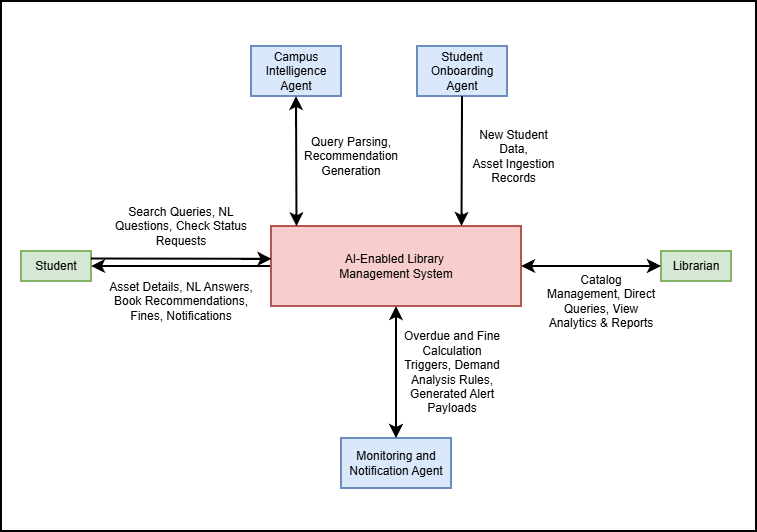
\includegraphics[width=0.88\textwidth]{Level_0_DFD.png}%
    }{%
        \fbox{\parbox{0.82\textwidth}{\centering
        Level 0 DFD image not found at the configured figure path.}}%
    }
    \caption{Level 0 Data Flow Diagram of the Smart Library Management System}
    \label{fig:level0}
\end{figure}

\begin{figure}[H]
    \centering
    \IfFileExists{Level_1_DFD.png}{%
        \includegraphics[width=0.88\textwidth]{Level_1_DFD.png}%
    }{%
        \fbox{\parbox{0.82\textwidth}{\centering
        Level 1 DFD image not found at the configured figure path.}}%
    }
    \caption{Level 1 Data Flow Diagram}
    \label{fig:level1}
\end{figure}

\begin{figure}[H]
    \centering
    \IfFileExists{Level_2_DFD.png}{%
        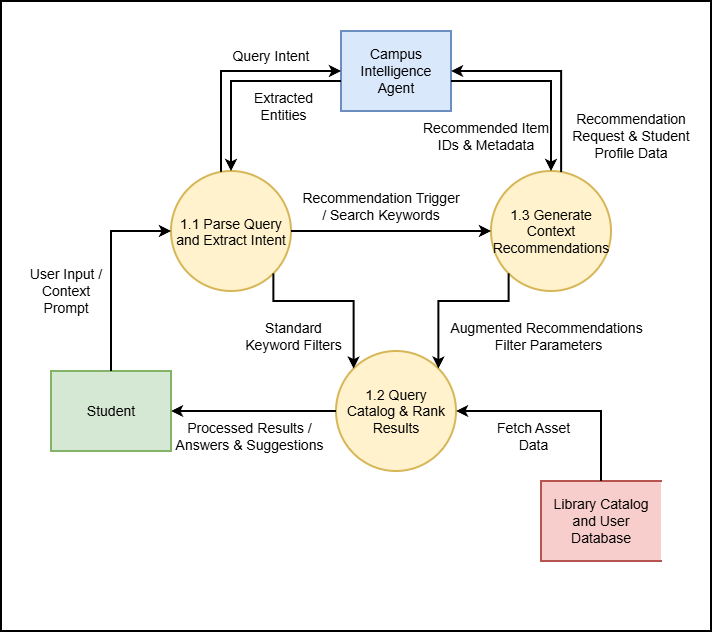
\includegraphics[width=0.88\textwidth]{Level_2_DFD.png}%
    }{%
        \fbox{\parbox{0.82\textwidth}{\centering
        Level 2 Data Flow Diagram}
        }%
    }
    \caption{Level 2 Data Flow Diagram}
    \label{fig:level2}
\end{figure}

\section{Technical Stack}

The prototype uses a single Python-oriented backend and AI stack to avoid
unnecessary technology fragmentation.

\begin{itemize}[leftmargin=0.7cm]
    \item \textbf{Frontend:} React.js with TypeScript and Tailwind CSS.
    \item \textbf{Backend:} FastAPI with Python 3.11+.
    \item \textbf{Database:} MySQL 8.0+.
    \item \textbf{ORM and database access:} SQLAlchemy with asynchronous
    MySQL connectivity.
    \item \textbf{AI integration:} LangChain with structured Pydantic
    outputs and OpenAI API integration.
    \item \textbf{Validation:} Pydantic models for API and agent data.
    \item \textbf{Duplicate detection:} RapidFuzz-based string similarity
    combined with deterministic Roll Number and ISBN checks.
    \item \textbf{Testing:} Pytest-based unit and integration testing.
    \item \textbf{Version control and CI/CD:} GitHub repository and automated
    CI checks for testing, linting, and build validation.
\end{itemize}

\section{Database Design}

The database extends the existing library schema with two operational
tables.

\subsection{Notification Queue}

The \texttt{NOTIFICATION\_QUEUE} table stores notifications generated by
overdue and other automated workflows. It references the student table and
supports notification types and processing states.

\subsection{Search Demand Logs}

The \texttt{SEARCH\_DEMAND\_LOGS} table records student search activity,
including the extracted category and timestamp. These records provide the
data required for later demand analysis and acquisition recommendations.

\subsection{Performance-Oriented Indexing}

Indexes are provided for frequently accessed search and monitoring fields.
In particular, composite indexes on
\texttt{ISSUING\_DETAILS(Status, Due\_Date)} and
\texttt{BOOKS(Category, Total\_Copies)} support overdue scanning and
inventory-oriented analysis.

\section{Implementation Details}

\subsection{Library Intelligence Agent}

The Library Intelligence Agent interprets a student's natural-language
request into a structured representation containing the intended operation,
search keywords, category, availability requirement, and confidence.

The prototype uses a Pydantic structured-output schema. The language model
does not receive database credentials or unrestricted SQL execution
capability. After interpretation, the backend performs parameterized
database queries and calculates real-time availability from catalog and
circulation data.

If the AI service is unavailable or confidence is below the configured
threshold, the system falls back to deterministic keyword-based search.
This preserves the basic resource-discovery workflow without making the
library dependent on an external AI service.

\subsection{Record Onboarding Agent}

The Record Onboarding Agent validates incoming student and catalog records
before insertion. Student records are checked using exact Roll Number and
email comparisons and, where necessary, fuzzy name similarity. Catalog
records use Asset ID and ISBN checks together with title/publisher
similarity.

Potential duplicates are skipped and reported rather than silently deleted.
The backend owns the database transaction, allowing the ingestion operation
to remain atomic.

\subsection{Library Monitoring Agent}

The Library Monitoring Agent performs deterministic overdue processing. It
identifies active loans whose due dates have passed, calculates the number
of overdue days, and updates or creates corresponding fine records.

The agent also creates entries in the notification queue so that overdue
students can be informed through a later notification-delivery mechanism.

A separate demand-analysis operation aggregates search-demand logs and
compares demand categories with low-inventory books. This produces
acquisition recommendations for library administrators.

\subsection{Controlled AI and Safety Model}

The prototype follows a strict separation between AI interpretation and
database modification:

\begin{itemize}[leftmargin=0.7cm]
    \item LLM outputs are constrained to Pydantic schemas.
    \item Database writes are performed by backend services.
    \item SQLAlchemy parameterization is used instead of string-concatenated
    SQL.
    \item Financial calculations are deterministic and are not delegated to
    the language model.
    \item AI failure does not prevent conventional keyword search.
    \item Potential onboarding duplicates are reported for review rather
    than automatically removed.
\end{itemize}

\section{Prototype Workflow}

The main student workflow is:

\begin{enumerate}[leftmargin=0.7cm]
    \item Student submits a natural-language resource request.
    \item The Library Intelligence Agent extracts the search intent and
    relevant terms.
    \item Backend services query the MySQL catalog using controlled,
    parameterized operations.
    \item Current issued copies are calculated from circulation records.
    \item Results are ranked using relevance and availability information.
    \item The search request and extracted category are logged for demand
    analysis.
\end{enumerate}

The administrator workflow similarly combines deterministic monitoring with
analytical assistance:

\begin{enumerate}[leftmargin=0.7cm]
    \item Overdue loans are identified from circulation records.
    \item Late days and fines are calculated deterministically.
    \item Fine records and notification entries are created or updated.
    \item Search-demand logs are aggregated by category.
    \item Categories with high demand and low inventory are surfaced as
    acquisition recommendations.
\end{enumerate}

% =====================================================
% CHAPTER 3
% =====================================================

\chapter{Results and Evaluation}

\section{Prototype Implementation Status}

The prototype implementation is organized around the incremental delivery
strategy established in the proposal. The current implementation baseline
contains the following major components:

\begin{table}[H]
\centering
\begin{tabularx}{\textwidth}{>{\raggedright\arraybackslash}p{4.2cm} X}
\toprule
\textbf{Component} & \textbf{Prototype Capability} \\
\midrule
Database extension &
Notification queue, search-demand logging, foreign keys, and performance-oriented indexes. \\

Backend API &
FastAPI endpoints for intelligent search, ingestion, fines, and overdue monitoring. \\

Intelligent search &
Structured natural-language interpretation with a deterministic keyword-search fallback. \\

Record onboarding &
Pydantic validation, duplicate checks, fuzzy similarity, and transactional insertion. \\

Fine management &
Real-time overdue-day calculation and outstanding-balance computation. \\

Monitoring &
Automated overdue scanning, fine updates, and notification generation. \\

Demand analysis &
Aggregation of search-demand categories against low-inventory catalog records. \\

Frontend &
React/TypeScript dashboard with natural-language search, loan/fine tracking, and librarian monitoring views. \\

Engineering controls &
Parameterized database access, controlled AI output, modular services, and automated testing structure. \\
\bottomrule
\end{tabularx}
\caption{Prototype implementation scope}
\label{tab:prototype-status}
\end{table}

\section{Testing Methodology}

The prototype evaluation follows multiple levels of testing.

\subsection{Unit Testing}

Individual components are tested independently. Examples include:

\begin{itemize}[leftmargin=0.7cm]
    \item validation of student records,
    \item rejection of invalid academic-year values,
    \item natural-language fallback parsing,
    \item overdue-day calculation, and
    \item deterministic fine calculation.
\end{itemize}

\subsection{Integration Testing}

Integration tests verify that API routes, service classes, database models,
and agent outputs work together. Important integration scenarios include
intelligent search followed by demand logging, bulk ingestion followed by
duplicate detection, and overdue monitoring followed by fine and
notification creation.

\subsection{Performance Testing}

Database indexes, pagination-oriented queries, and API response times are
evaluated against the proposal's performance objectives. The primary
engineering target is to keep common API operations within the proposed
response-time budget while maintaining correctness.

\subsection{Functional Testing}

Representative library scenarios are used to validate:

\begin{enumerate}[leftmargin=0.7cm]
    \item resource search with a natural-language request,
    \item availability-aware search,
    \item duplicate student ingestion,
    \item duplicate catalog ingestion,
    \item active overdue loans,
    \item fine calculation,
    \item notification generation, and
    \item high-demand/low-availability detection.
\end{enumerate}

\section{Evaluation Metrics}

The proposal defines measurable targets for the complete system. At the
prototype stage, these metrics are treated as evaluation criteria rather
than as claims of achieved performance.

\begin{table}[H]
\centering
\begin{tabularx}{\textwidth}{>{\raggedright\arraybackslash}p{5.1cm} >{\centering\arraybackslash}p{3cm} X}
\toprule
\textbf{Metric} & \textbf{Target} & \textbf{Prototype Evaluation Status} \\
\midrule
Resource discovery time & $\leq 10$ s &
To be measured using predefined resource queries. \\

Duplicate detection precision & $\geq 90\%$ &
To be measured using a labeled duplicate/non-duplicate dataset. \\

Overdue detection coverage & $\geq 99\%$ &
To be measured against controlled overdue scenarios. \\

Demand recommendation accuracy & $\geq 90\%$ &
To be measured against labeled or synthetic demand cases. \\

Median API response time & $\leq 500$ ms &
To be measured under representative database load. \\

AI answer validity & $\geq 90\%$ &
To be evaluated against grounded catalog responses. \\

Automated test coverage & $\geq 70\%$ &
To be measured from the completed test suite. \\

Deployment availability & $\geq 99\%$ &
To be evaluated after deployment and monitoring are established. \\
\bottomrule
\end{tabularx}
\caption{Prototype and final-system evaluation criteria}
\label{tab:evaluation}
\end{table}

No numerical performance result is claimed here without measurement. The
purpose of the prototype stage is to establish the mechanisms needed to
collect reproducible measurements during subsequent evaluation.

\section{Analysis}

The prototype architecture provides several engineering benefits.

First, deterministic library operations remain independent of the AI
service. This is particularly important for fines, overdue status,
circulation transactions, and database writes because these operations
require predictable and auditable behavior.

Second, the AI layer is constrained to structured interpretation and
analysis. This reduces the risk of hallucinated resource information being
treated as authoritative database data.

Third, the keyword-search fallback preserves basic functionality when the
AI service is unavailable or produces a low-confidence interpretation. This
supports the proposal's requirement that the project remain practically
usable rather than depending entirely on an external model.

Finally, the search-demand logging mechanism creates a feedback loop between
student behavior and administrative decision support. Repeated searches can
be analyzed together with inventory levels to identify potential acquisition
needs.

% =====================================================
% CHAPTER 4
% =====================================================

\chapter{Conclusion}

\section{Summary of Work}

The prototype establishes the engineering foundation for the
AI-Enabled Smart Library Management and Resource Recommendation System.
The design integrates a React/TypeScript frontend, FastAPI backend, MySQL
database, and controlled multi-agent AI layer.

The implementation is organized into separate services for intelligent
resource discovery, record onboarding, circulation/fine handling, overdue
monitoring, and demand analysis. The database design extends the core
library schema with notification and search-demand logging capabilities.

The prototype follows the project's time-to-value strategy by prioritizing
working library workflows and then adding AI-assisted functionality in
modular increments.

\section{Key Findings}

\begin{itemize}[leftmargin=0.7cm]
    \item \textbf{AI should assist rather than control deterministic
    workflows:} Search interpretation and analytical recommendations benefit
    from AI, while fines, due dates, and database transactions should remain
    under deterministic backend control.

    \item \textbf{Fallback behavior is essential:} Keyword-based search
    provides continued resource discovery when the AI service is unavailable
    or uncertain.

    \item \textbf{Demand logging adds operational value:} Search activity
    can be transformed into a measurable input for high-demand,
    low-availability analysis.

    \item \textbf{Modular architecture supports incremental development:}
    The separation of agents, backend services, database models, and frontend
    components allows additional functionality to be introduced without
    redesigning the complete system.
\end{itemize}

\section{Future Work and Recommendations}

The following work is planned for subsequent iterations:

\begin{enumerate}[leftmargin=0.7cm]
    \item Complete and validate the full student and administrator
    authentication and role-based access-control workflow.
    \item Expand natural-language recommendations using availability-aware
    retrieval and richer catalog metadata.
    \item Complete bulk student and catalog onboarding with CSV ingestion,
    review workflows, and larger duplicate-detection evaluation datasets.
    \item Integrate notification delivery for queued overdue messages.
    \item Extend demand analysis into administrator dashboards and
    purchase-priority reports.
    \item Conduct controlled performance testing to measure the proposed
    response-time and reliability targets.
    \item Increase automated unit and integration test coverage and integrate
    the test suite into CI/CD.
    \item Containerize the system and validate deployment in a staging
    environment before final production deployment.
\end{enumerate}

\section{Final Remarks}

The prototype demonstrates the intended engineering direction of the project:
a practical library-management platform enhanced by carefully controlled AI
rather than an AI research system. The architecture emphasizes rapid
incremental delivery, measurable evaluation, reliable database operations,
fallback behavior, and future scalability.

The next development stages will focus on integrating the individual
components into a complete end-to-end workflow and collecting quantitative
evaluation results. These measurements will determine whether the system
meets the targets defined in the project proposal.

\end{document}
